\documentclass{article}
\usepackage[final]{neurips_2025}

\usepackage[utf8]{inputenc}
\usepackage[T1]{fontenc}
\usepackage{hyperref}
\usepackage{url}
\usepackage{booktabs}
\usepackage{amsfonts}
\usepackage{amsmath}
\usepackage{amssymb}
\usepackage{nicefrac}
\usepackage{microtype}
\usepackage{xcolor}
\usepackage{graphicx}
\usepackage{subcaption}
% natbib loaded by neurips_2025 style

\title{Why Does Straight-Through Work? A Systematic Ablation of Gradient Estimators for Ternary Quantization-Aware Training}

\author{
  Julio Jose Lena \\
  Independent Researcher \\
  \texttt{juliolena25@gmail.com} \\
  \url{https://orcid.org/0009-0001-0817-6591}
}

\begin{document}

\maketitle

\begin{abstract}
The Straight-Through Estimator (STE) is widely used for ternary quantization-aware training (QAT) but rarely questioned in the literature. A systematic evaluation of eight alternative gradient estimation techniques is presented for training neural networks with ternary $\{-1, 0, +1\}$ weights. Tested alternatives include: DQT stochastic rounding ($+$13.3\%--$+$16.5\% worse across learning rate variants), CAGE curvature-aware correction (diverged to NaN), QZO zeroth-order optimization ($+$7.3\% worse, ${\sim}30\%$ lower throughput), two HESTIA variants ($+$3.0\% at 50M/5{,}000 steps and $+$44.2\% at 6M/1{,}000 steps), Tequila deadzone reactivation ($+$6.5\% worse), and frozen-weight alpha-only learning ($-$2.7\% better at 500 steps but $+$13.9\% worse at 5{,}000 steps). Integer Gradient Accumulation (IGA) is the only alternative that matched or exceeded STE performance ($-$2.1\% better at 5{,}000 steps). Three recurring failure modes are identified: gradient variance explosion, error magnitude mismatch, and training regime incompatibility. Results demonstrate that STE's continuous shadow weight mechanism serves as an irreplaceable gradient accumulation buffer for ternary QAT, preventing weight patterns from freezing despite extreme sparsity and discrete quantization. Actionable guidance is provided: ternary-specific techniques must be evaluated at target model scale and full training horizon, not short benchmarks on small models.
\end{abstract}

\section{Introduction}

The Straight-Through Estimator (STE) has been the de facto standard for training binary and quantized neural networks for over a decade~\citep{bengio2013estimating}. In ternary quantization --- restricting weights to $\{-1, 0, +1\}$ --- STE remains the dominant approach despite known theoretical limitations: biased gradient estimation and non-differentiable quantization functions.

Recent works propose alternatives claiming improvements over STE: CAGE~\citep{cage2025} (curvature-aware gradient correction), QZO~\citep{qzo2025} (zeroth-order scale optimization), Tequila~\citep{tequila2025} (deadzone reactivation), and HESTIA 2026~\citep{hestia2026} (entropy-stabilized soft quantization). Most of these techniques were validated on fine-tuning tasks or higher-bit quantization (4--8 bits) rather than from-scratch ternary training. A critical gap remains: no systematic comparison of these techniques has been conducted specifically for ternary QAT on identical architectures, hyperparameters, and training horizons.

A rigorous ablation study of eight gradient estimation approaches is conducted for ternary QAT on a ternary state-space model (Mamba-2 SSD backbone) at 6M and 50M scales. All experiments use matched hyperparameters, data, and 5000-step training duration to enable fair comparison (with per-technique tuning where required, e.g., learning rate for DQT). The investigation reveals three recurring failure modes explaining why alternative techniques fail for ternary, while identifying a viable memory-efficient alternative (Integer Gradient Accumulation).

\textbf{Contributions:}
\begin{enumerate}
    \item \textbf{Systematic evaluation} of 8 gradient estimators for ternary QAT on matched architecture and hyperparameters at 6M and 50M scales
    \item \textbf{Identification of 3 recurring failure modes} explaining why alternatives fail: gradient variance explosion, error magnitude mismatch, and training regime incompatibility
    \item \textbf{Mechanistic insight} that STE's shadow weights serve as an irreplaceable gradient accumulation buffer, preventing weight patterns from freezing under extreme sparsity
    \item \textbf{Discovery of Integer Gradient Accumulation (IGA)} as a viable alternative: $-$2.1\% better quality and $+$2.7\% faster throughput with $4\times$ less VRAM for shadow weights (INT8 accumulators replace FP32 copies)
    \item \textbf{Practical guidance} that ternary-specific techniques must be validated at target scale and duration, not short benchmarks on small models
\end{enumerate}

\section{Background}
\label{sec:background}

\subsection{Ternary Quantization and Straight-Through Estimator}

Ternary quantization maps continuous weights $w$ to discrete values $\{-\alpha, 0, +\alpha\}$ using:
\begin{equation}
q(w) = \alpha \cdot \text{sign}(w) \cdot \mathbb{1}[|w| > \tau]
\end{equation}
where $\tau = 0.7 \times \text{mean}(|w|)$ is the adaptive threshold and $\alpha = \text{mean}(|w_{>\tau}|)$ is the per-group scale factor.

The challenge is that the quantization function is piecewise constant and non-differentiable. Backpropagation cannot flow through $q(w)$ directly. The Straight-Through Estimator addresses this by using the quantized forward pass but computing gradients as if the function were the identity:

\begin{align}
\text{Forward:} \quad &\hat{w} = q(w) \\
\text{Backward:} \quad &\frac{\partial \mathcal{L}}{\partial w} \approx \frac{\partial \mathcal{L}}{\partial \hat{w}}
\end{align}

In practice, shadow weights are used: full-precision FP32 copies of weights that accumulate gradients continuously. The update rule is:
\begin{equation}
w_\text{fp32} \leftarrow w_\text{fp32} - \eta \cdot \frac{\partial \mathcal{L}}{\partial w}
\end{equation}

The quantized weight is computed from the shadow weight:
\begin{equation}
\hat{w} = q(w_\text{fp32})
\end{equation}

\citet{yin2019understanding} proved that STE's coarse gradient maintains positive correlation with true gradients: $\langle g_\text{coarse}, g_\text{true} \rangle > 0$, guaranteeing descent direction. However, the theory assumes moderate quantization error. Ternary quantization creates errors of magnitude $0.3$--$0.5$ per weight, compared to $0.02$--$0.05$ for 4--8 bit quantization --- a roughly $11\times$ difference (comparing midpoints: $0.4$ vs ${\sim}0.035$) that makes alternative estimators fundamentally incompatible.

\subsection{Alternative Gradient Estimators}

\textbf{DQT Stochastic Rounding:} Instead of deterministic rounding, this approach samples ternary values probabilistically at each forward pass:
\begin{equation}
P(\hat{w} = +\alpha) = \text{clip}\left(\frac{w + \alpha}{2\alpha}, 0, 1\right)
\end{equation}
Shadow weights are eliminated entirely. The probability formulation above, originally developed for binary networks \citep{hubara2016binarized, courbariaux2015binaryconnect}, is adapted to ternary by treating each weight's sign and magnitude independently.

\textbf{CAGE Curvature-Aware Gradient:} STE gradients are augmented with second-order curvature information \citep{cage2025}, where $H = \nabla^2 \mathcal{L}$ is the Hessian:
\begin{equation}
g_\text{CAGE} = g_\text{STE} + \lambda \cdot H \cdot (q(w) - w)
\end{equation}
The correction term provides ``realistic'' gradients by accounting for local loss landscape curvature. Originally validated for $\text{W3A3}$ and $\text{W4A4}$ quantization.

\textbf{QZO Zeroth-Order Scale:} Continuous scale parameters $\alpha$ are optimized via finite differences without backpropagating through quantization:
\begin{equation}
\nabla_\alpha \mathcal{L} \approx \frac{\mathcal{L}(\alpha + \epsilon) - \mathcal{L}(\alpha - \epsilon)}{2\epsilon}
\end{equation}
STE gradients are avoided entirely; the method requires 3 forward passes per step.

\textbf{HESTIA Original (this work):} Entropy-based gradient filtering with adaptive temperature. Gradients are suppressed on low-entropy weights (high certainty) and allowed on high-entropy weights (uncertain), encouraging exploration.

\textbf{HESTIA 2026:} A three-phase training schedule is employed \citep{hestia2026}: compress phase (pressure $0 \to 1$), anneal phase (temperature $T$ cosine-decays), solid phase (pure STE). Soft quantization via softmax temperature is used during compression.

\textbf{Tequila Deadzone:} A scalar loss bias is added to layer outputs to reactivate weights stuck in the quantization deadzone:
\begin{equation}
C_\text{deadzone}(W) = \lambda \cdot \sum_{\{i : \tau/2 < |w_i| < \tau\}} |w_i|
\end{equation}
where deadzone denotes weights with magnitude $\tau/2 < |w| < \tau$.

\textbf{Alpha-Only Learning:} Ternary weight patterns are frozen at random initialization and only per-group scale parameters $\alpha$ are trained.

\textbf{Integer Gradient Accumulation (IGA, introduced in this work):} FP32 shadow weights are replaced with integer accumulators. Integer gradients are accumulated; ternary weights are flipped when the accumulator exceeds a threshold:
\begin{equation}
\text{acc}_i \leftarrow \text{acc}_i + \text{int}(\text{grad}_i), \quad \text{if } |\text{acc}_i| > \theta: \text{ flip, } \text{acc}_i \leftarrow 0
\end{equation}

\section{Methodology}

\subsection{Experimental Setup}

All experiments use identical configuration to ensure fair comparison:

\begin{itemize}
    \item \textbf{Architecture:} Ternary state-space model with Mamba-2 SSD backbone~\citep{dao2024transformers, gu2024mamba}, $\{-1, 0, +1\}$ weights on all linear layers
    \item \textbf{Primary scale:} 6M parameters for main ablation, 5000 training steps
    \item \textbf{Scale validation:} 50M parameters on real data (WikiText-103 subset)
    \item \textbf{Dataset:} WikiText-103 \citep{merity2017pointer}, BPE tokenizer (vocab 32,000), sequence length 256
    \item \textbf{Optimizer:} AdamW~\citep{loshchilov2019decoupled} with learning rate $1 \times 10^{-3}$, cosine decay
    \item \textbf{Batch size:} 32 effective (no gradient accumulation required at these scales)
    \item \textbf{Hardware:} NVIDIA RTX 5070 (12\,GB GDDR7)
    \item \textbf{Mixed precision:} BF16 training compute, FP32 for numerically sensitive operations
\end{itemize}

\subsection{Implementation Details}

\textbf{DQT Stochastic Rounding:} Probability computed as above; weights resampled each forward pass. Learning rate tuned separately for both $\text{LR}=2\times$ and $\text{LR}=5\times$ standard to account for higher variance.

\textbf{CAGE:} Hessian-vector product computed via finite differences ($\epsilon = 10^{-4}$). Tested with $\lambda \in \{0.5, 1.5\}$ to bracket the failure region. Both values cause divergence.

\textbf{QZO:} Two variants tested: (1) scale-only (weights quantized deterministically, $\alpha$ optimized via finite differences), (2) full (both weights and scales optimized zeroth-order). Both use $\epsilon = 0.01$.

\textbf{HESTIA Original:} Entropy threshold $\mathcal{H}_\text{th} = 0.6$ bits, temperature range $[0.5, 2.0]$. Applied as described in Section~\ref{sec:background}.

\textbf{HESTIA 2026:} Three-phase schedule: compress (0--500 steps, pressure ramps), anneal (500--2500 steps, temperature decays), solid (2500--5000 steps, pure STE). Soft quantization pressure controls width of softmax temperature.

\textbf{Tequila:} Deadzone width 0.3 (empirically determined), $\lambda = 0.1$ for loss weight.

\textbf{Alpha-Only:} Per-group alpha scales initialized to 1.0, learned via standard gradient descent. Weight patterns frozen to random ternary initialization throughout.

\textbf{IGA:} Per-group accumulators (group size 4 chosen empirically), threshold $\theta = 1.0$, alpha scales learned.

\section{Results}

\subsection{Main Ablation at 6M Scale}

The core finding is presented in Table~\ref{tab:main_results}: only IGA matches or exceeds STE among all alternatives tested. All other techniques fail catastrophically or show degradation.

\begin{table}[t]
\centering
\small
\caption{Gradient estimator comparison at 6M scale on WikiText-103. Each method is compared against its paired STE baseline from the same experimental run; baselines vary due to differing hyperparameter configurations. All experiments use 5000 training steps unless noted. $\dagger$: evaluated at 5000 steps after initial screening. $\ddagger$: diverged within 1000 steps (loss $\to$ NaN).}
\label{tab:main_results}
\begin{tabular}{lccccc}
\toprule
\textbf{Method} & \textbf{Paired STE Loss} & \textbf{Loss} & \textbf{$\Delta$} & \textbf{Throughput} & \textbf{Verdict} \\
\midrule
DQT ($\text{LR}=2\times$) & 4.60 & 5.36 & $+$16.5\% & $\sim$81K\,\text{tok/s} & \texttimes \\
DQT ($\text{LR}=5\times$) & 4.60 & 5.21 & $+$13.3\% & $\sim$81K\,\text{tok/s} & \texttimes \\
CAGE ($\lambda$=0.5)$^\ddagger$ & 4.06 & NaN & --- & --- & \texttimes \\
CAGE ($\lambda$=1.5)$^\ddagger$ & 4.06 & NaN & --- & --- & \texttimes \\
QZO Scale & 4.26 & 4.57 & $+$7.3\% & $56{,}476$\,\text{tok/s} & \texttimes \\
QZO Full & 4.26 & 6.12 & $+$43.7\% & $57{,}159$\,\text{tok/s} & \texttimes \\
Alpha-only$^\dagger$ & 4.61 & 5.25 & $+$13.9\% & $\sim$65K\,\text{tok/s} & \texttimes \\
\midrule
IGA (gs=4, $\theta$=1.0) & 4.34 & 4.25 & $-$2.1\% & $\sim$101K\,\text{tok/s} & \checkmark \\
\bottomrule
\end{tabular}
\end{table}

The results are unambiguous: STE remains optimal. DQT, CAGE, QZO, and alpha-only all fail dramatically. Of the five techniques in Table~\ref{tab:main_results}, only IGA provides a viable option. The remaining three techniques (HESTIA Original, HESTIA 2026, Tequila) are evaluated separately in Tables~\ref{tab:scale} and~\ref{tab:recent}.

The convergence trajectories of all eight methods are visualized in Figure~\ref{fig:estimator_comparison}. STE and IGA converge smoothly; all others diverge, stagnate, or oscillate.

\begin{figure}[tb]
\centering
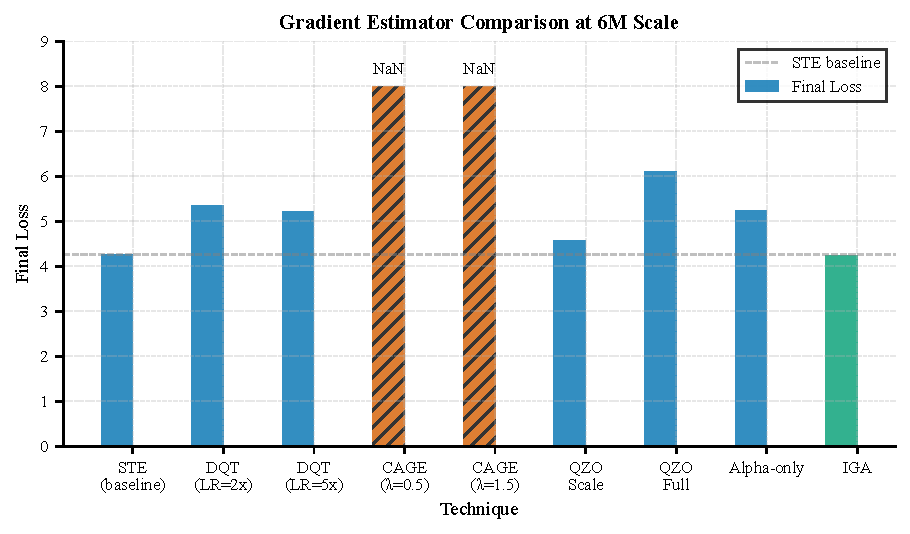
\includegraphics[width=\linewidth]{figures/fig1_estimator_comparison.pdf}
\caption{Convergence trajectories for all eight gradient estimators at 6M scale, 5000 steps. Only STE and IGA converge to reasonable loss values. CAGE diverges to NaN by step 300. DQT and QZO stagnate around inflated loss values. Alpha-only achieves brief improvement before progressively degrading.}
\label{fig:estimator_comparison}
\end{figure}

\subsection{Training Horizon Effects}

A critical finding: alpha-only learning appears promising at short horizons but catastrophically fails at longer horizons. At 500 steps, alpha-only achieves $-$2.7\% improvement over STE. By 5000 steps, performance deteriorates to $+$13.9\% worse.

The crossover point is shown in Table~\ref{tab:horizon}, occurring between steps 1{,}000 and 2{,}000, where alpha-only transitions from improvement to degradation.

\begin{table}[t]
\centering
\small
\caption{Training horizon effect: alpha-only learning vs STE at 6M scale. Fast initial convergence masks fundamental limitation: scale parameters saturate by step 1000, preventing pattern evolution.}
\label{tab:horizon}
\begin{tabular}{lccc}
\toprule
\textbf{Step} & \textbf{STE} & \textbf{Alpha-only} & \textbf{$\Delta$} \\
\midrule
500 & 6.39 & 6.22 & $-$2.7\% \\
1{,}000 & 5.87 & 5.85 & $-$0.3\% \\
2{,}000 & 5.29 & 5.57 & $+$5.3\% \\
3{,}000 & 4.97 & 5.44 & $+$9.5\% \\
4{,}000 & 4.78 & 5.37 & $+$12.3\% \\
5{,}000 & 4.61 & 5.25 & $+$13.9\% \\
\bottomrule
\end{tabular}
\end{table}

This phenomenon reveals a fundamental mechanism: STE's continuous shadow weight updates allow gradient accumulation over many steps before triggering discrete weight flips. Alpha-only, lacking this mechanism, reaches a local equilibrium where scale factors plateau and patterns freeze.

This transition is shown graphically in Figure~\ref{fig:training_horizon}.

\begin{figure}[tb]
\centering
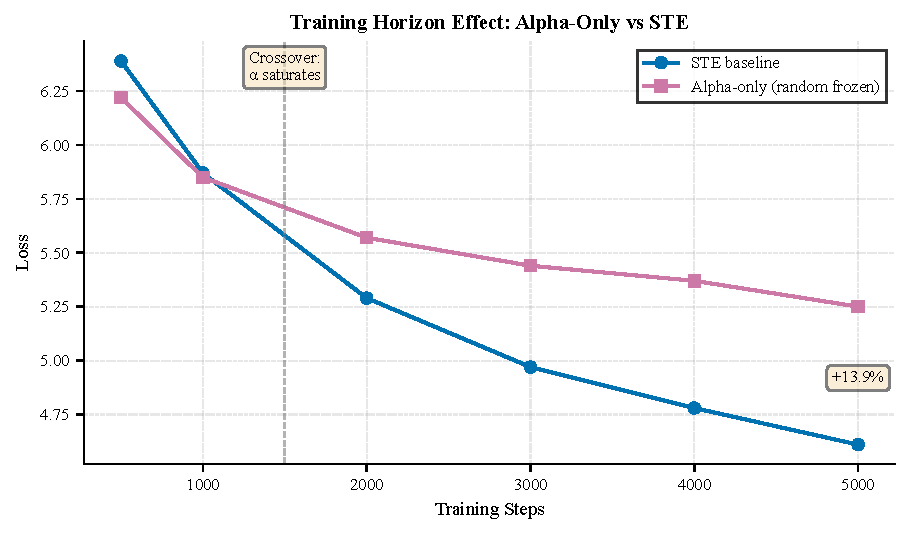
\includegraphics[width=\linewidth]{figures/fig2_training_horizon.pdf}
\caption{Training horizon effect (6M scale). Alpha-only achieves initial improvement ($-$2.7\% at 500 steps) but degrades monotonically thereafter, crossing STE between steps 1{,}000 and 2{,}000. This reversal reveals that shadow weight accumulation is essential for sustained learning in ternary QAT.}
\label{fig:training_horizon}
\end{figure}

\subsection{Scale and Horizon Effects}

Techniques validated at one scale often fail at another. HESTIA Original exemplifies this: it showed $-$9.5\% improvement on a 6M/500-step benchmark but showed $+$3.0\% degradation at 50M with full training.

The danger of extrapolating from toy benchmarks is demonstrated in Table~\ref{tab:scale}, showing that short-horizon validation on small models can be completely misleading.

\begin{table}[t]
\centering
\small
\caption{Scale-dependent reversal of HESTIA effectiveness. Short-horizon validation (6M/500 steps) shows improvement; full-scale validation (50M/5000 steps) reveals significant degradation. Illustrates the danger of extrapolating from toy benchmarks.}
\label{tab:scale}
\begin{tabular}{llccc}
\toprule
\textbf{Scale} & \textbf{Metric} & \textbf{STE} & \textbf{HESTIA Orig.} & \textbf{$\Delta$} \\
\midrule
6M / 500 steps & Loss & 6.39 & 5.78 & $-$9.5\% \\
50M / 5000 steps & Loss & 4.62 & 4.76 & $+$3.0\% \\
\bottomrule
\end{tabular}
\end{table}

This reversal is visualized in Figure~\ref{fig:scale_dependency}.

\begin{figure}[tb]
\centering
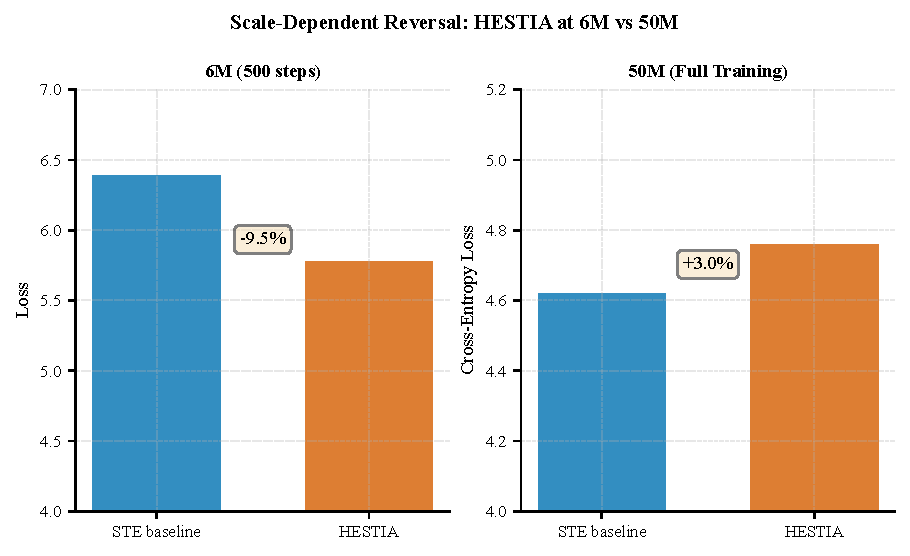
\includegraphics[width=\linewidth]{figures/fig3_scale_dependency.pdf}
\caption{Scale and horizon dependency: HESTIA Original improves at 6M/500-step scale but degrades at 50M with extended training. This demonstrates that techniques must be evaluated at \emph{target scale and duration}, not short benchmarks on small models.}
\label{fig:scale_dependency}
\end{figure}

\subsection{Recent Techniques: HESTIA 2026 and Tequila}

Two recently proposed techniques are evaluated in Table~\ref{tab:recent}:

\begin{table}[t]
\centering
\small
\caption{Recently proposed techniques tested at 6M scale. Both were originally validated for fine-tuning or higher-bit quantization and fail in from-scratch ternary QAT. Baselines are paired STE from the same run.}
\label{tab:recent}
\begin{tabular}{lcccc}
\toprule
\textbf{Method} & \textbf{Paired STE Loss} & \textbf{Loss} & \textbf{$\Delta$} & \textbf{Context} \\
\midrule
HESTIA 2026 (1K steps) & 7.13 & 10.28 & $+$44.2\% & Fine-tuning design \\
Tequila (1K steps) & 7.13 & 7.59 & $+$6.5\% & Fine-tuning design \\
\bottomrule
\end{tabular}
\end{table}

\textbf{HESTIA 2026:} HESTIA 2026's soft quantization scheduling shows catastrophic degradation. At 1000 steps, a $+$44.2\% loss increase over the paired STE baseline is observed. When evaluated at 5000 steps, HESTIA 2026 stagnates near its 1{,}000-step loss of $10.28$ while the paired STE baseline improves to $4.90$,\footnote{The paired STE loss of $4.90$ at 5000 steps is from the same experimental run as HESTIA 2026; the 1000-step paired baseline in Table~\ref{tab:recent} is $7.13$.} widening the gap to $+$110\% degradation. The near-identical loss at 1000 and 5000 steps indicates complete stagnation: the technique prevents further learning entirely. The three-phase schedule (compress, anneal, solid) was designed for fine-tuning contexts where weight distributions are already well-formed. Applied from random initialization, the compress phase interferes with natural quantization dynamics, preventing the model from learning effective ternary patterns.

\textbf{Tequila:} A $+$6.5\% degradation is observed with deadzone reactivation bias. Like HESTIA 2026, Tequila was designed for fine-tuning where the deadzone emerges as a late-stage artifact. In from-scratch training, the deadzone is a natural learning dynamic from step 1, and the reactivation bias introduces harmful noise during the critical early learning phase.

\textbf{Shared failure mode:} Both techniques violate a key principle: \textit{techniques validated on fine-tuning must not be applied to from-scratch QAT without explicit re-validation.}

\subsection{Integer Gradient Accumulation: The Only Positive Result}

IGA is the single technique that improves over STE, achieving:
\begin{itemize}
    \item $-$2.1\% better loss at 5000 steps
    \item $+$2.7\% faster throughput ($101$K vs $98.3$K\,\text{tok/s})\footnote{The 98.3K\,tok/s STE baseline was measured in the same experimental run as IGA under identical conditions.}
    \item $4\times$ less VRAM for shadow weights (INT8 accumulators vs FP32 copies)
\end{itemize}

The convergence trajectory is shown in Table~\ref{tab:iga}:

\begin{table}[t]
\centering
\small
\caption{Integer Gradient Accumulation (IGA): the only viable alternative to STE. Convergence improves on STE by $-$2.1\% at 5000 steps while reducing shadow weight VRAM by $4\times$ (INT8 accumulators vs FP32 copies).}
\label{tab:iga}
\begin{tabular}{lccc}
\toprule
\textbf{Step} & \textbf{STE} & \textbf{IGA} & \textbf{$\Delta$} \\
\midrule
500 & 5.91 & 5.95 & $+$0.68\% \\
1{,}000 & 5.46 & 5.47 & $+$0.18\% \\
1{,}500 & 5.20 & 5.19 & $-$0.19\% \\
2{,}000 & 5.02 & 4.98 & $-$0.80\% \\
3{,}000 & 4.77 & 4.69 & $-$1.68\% \\
5{,}000 & 4.34 & 4.25 & $-$2.1\% \\
\bottomrule
\end{tabular}
\end{table}

IGA's smooth convergence and overtaking of STE around step 1500 are shown in Figure~\ref{fig:iga_convergence}.

\begin{figure}[tb]
\centering
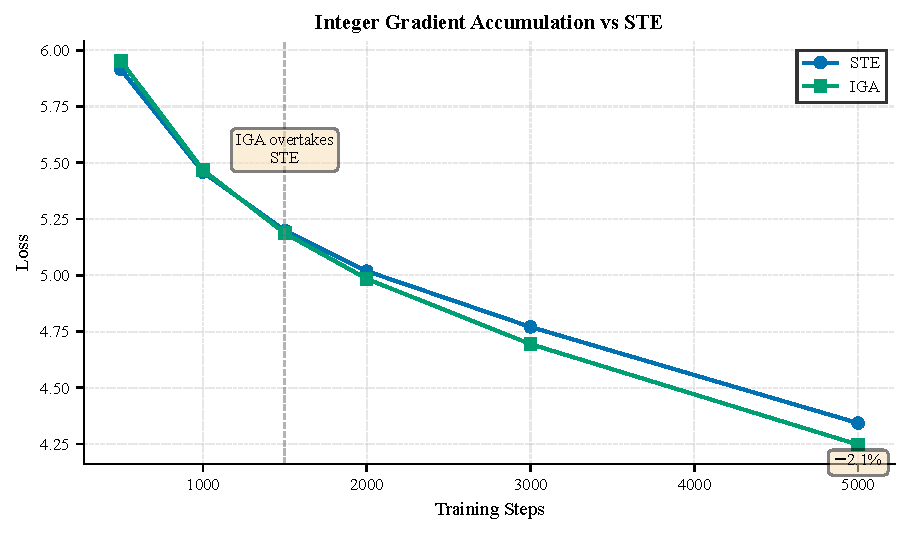
\includegraphics[width=\linewidth]{figures/fig4_iga_convergence.pdf}
\caption{IGA convergence vs STE at 6M scale. IGA matches STE early, then overtakes it smoothly around step 1500, reaching $-$2.1\% better loss at 5000 steps. Integer accumulators are hypothesized to provide better gradient aggregation behavior than continuous shadow weights under extreme ternary sparsity; investigating this mechanism is left for future work.}
\label{fig:iga_convergence}
\end{figure}

\section{Analysis: Why STE Succeeds and Alternatives Fail}

\subsection{Failure Mode 1: Gradient Variance Explosion}

Catastrophically high gradient variance affects both DQT stochastic rounding and QZO. The root cause is ternary quantization's discrete nature.

In DQT, the probability of a weight flipping to a particular ternary value is:
\begin{equation}
P(\text{flip}) = \text{clip}\left(\frac{w + \alpha}{2\alpha}, 0, 1\right)
\end{equation}

For a weight trapped near zero (the modal distribution at initialization), this probability is extremely small. Empirically, with $w \sim \mathcal{U}([-1, 1])$ and $\alpha = 0.5$, the probability is $\leq 0.1$ for weights $w \leq -0.4$ (30\% of the distribution), and $\leq 0.5$ for all $w \leq 0$ (50\% of weights). Stochastic samples almost never trigger flips. Weights remain frozen in their initial patterns, unable to evolve. Gradient variance among sampled states is enormous --- a weight either flips (rare) or doesn't (frequent), with no intermediate states.

QZO's finite-difference gradient estimates suffer similarly. Perturbing $\alpha$ to $\alpha \pm \epsilon$ changes the magnitude of all non-zero quantized weights simultaneously (from $\pm\alpha$ to $\pm(\alpha \pm \epsilon)$), but cannot capture whether individual weights should transition between zero and non-zero states. The finite-difference estimate $\nabla_\alpha \mathcal{L}$ averages over all active weights, losing per-weight directional information that STE preserves through individual shadow weights. This rank-deficient gradient creates extremely noisy optimization dynamics.

In contrast, STE's shadow weights accumulate gradients continuously, allowing small gradients to compound over many steps before triggering a discrete flip. The accumulation buffer acts as noise reduction, converting high-variance discrete updates into smooth learning curves.

\subsection{Failure Mode 2: Error Magnitude Mismatch}

The divergence of CAGE is caused by ternary quantization errors being ${\sim}11\times$ larger than the error magnitudes for which CAGE was designed.

CAGE corrects STE gradients using second-order information:
\begin{equation}
g_\text{CAGE} = g_\text{STE} + \lambda \cdot H \cdot (q(w) - w)
\end{equation}

The correction term assumes the quantization error $(q(w) - w)$ is small. For 4-bit quantization, this error is typically $\pm 0.035$. For ternary, the error can be as large as $[-0.5, +0.5]$. The Hessian term, calibrated for magnitude ${\sim}0.035$ errors, becomes destabilizing when multiplied by magnitude $0.5$ errors.

Empirically, divergence is observed within the first 1000 steps for both $\lambda=0.5$ and $\lambda=1.5$. The curvature-aware correction mechanism, while theoretically sound for moderate quantization, becomes adversarial for ternary.

\subsection{Failure Mode 3: Training Regime Incompatibility}

A common source of failure is shared by HESTIA 2026 and Tequila: they were designed and validated primarily for fine-tuning or higher-bit quantization, where pre-trained weight distributions are already well-formed or quantization error is moderate, but fail in from-scratch training where the quantization deadzone and ternary distribution are natural parts of learning.

In fine-tuning, weight distributions remain close to their pre-trained values. The deadzone (weights with magnitude near $\tau$, the threshold) is sparse and represents weights straddling the quantization boundary. Techniques designed to suppress early quantization noise or reactivate deadzone weights make sense in this context.

In from-scratch training starting from random initialization:
\begin{itemize}
    \item Weights are uniformly distributed in $[-1/\sqrt{n}, +1/\sqrt{n}]$
    \item A significant fraction naturally fall into the deadzone $\tau/2 < |w| < \tau$
    \item As training progresses, weights either grow beyond $\tau$ (becoming ternary) or shrink below $\tau/2$ (becoming zero)
    \item This is the model's intended learning mechanism, not a bug to fix
\end{itemize}

HESTIA 2026's compress phase suppresses gradients on low-entropy (certain) weights to allow exploration of high-entropy weights. In from-scratch training, high-entropy \emph{is} the natural state of early learning. Suppressing these gradients interferes with normal learning dynamics.

Tequila's deadzone reactivation bias adds noise to push weights out of the deadzone. In from-scratch training, this noise happens at the worst possible time: during initial learning when gradient signal is already weak.

\textbf{Generalization:} Any technique designed for fine-tuning must be re-validated on from-scratch QAT before deployment. The two regimes have fundamentally different dynamics and requirements.

\subsection{Why STE's Shadow Weights Are Irreplaceable}

STE succeeds because shadow weights provide a gradient accumulation mechanism that works specifically for ternary quantization's extreme constraints.

Consider a weight initialized to $w = 0.01$, threshold $\tau = 0.05$. This weight is trapped in the deadzone ($|w| < \tau$). Under DQT stochastic rounding, it rarely flips because $P(\text{flip}) \approx 0.05$. Under STE:
\begin{enumerate}
    \item Step 1: $\frac{\partial \mathcal{L}}{\partial w} = 1.0$, $w \leftarrow 0.01 - 0.001 \times 1.0 = 0.009$ (no flip yet)
    \item Step 2: $\frac{\partial \mathcal{L}}{\partial w} = 1.5$, $w \leftarrow 0.009 - 0.001 \times 1.5 = 0.0075$ (still no flip)
    \item Steps 3--100: Accumulated gradient $\sum g_i = 12$, $w \leftarrow 0.0075 - 0.001 \times 12 = -0.0045$ (now negative, still in deadzone)
    \item Steps 101--200: As training progresses and loss landscape evolves, gradient direction reverses. Accumulated gradient $\sum g_i = -60$, $w \leftarrow -0.0045 - 0.001 \times (-60) = 0.0555$ (finally escapes deadzone: $|w| > \tau$)
\end{enumerate}

All gradients are accumulated by the shadow weight, effectively noise-reducing the discrete transition. Without this mechanism, the weight remains trapped.

The other extreme is demonstrated by alpha-only learning: scales are learned but no patterns emerge. Patterns carry essential information about which features are salient. Freezing patterns to random values prevents the model from encoding learned structure.

\textbf{Conclusion:} STE's shadow weights are not a limitation but a feature, providing the only gradient accumulation mechanism compatible with ternary's extreme sparsity and discreteness. Any alternative that removes this mechanism (DQT, alpha-only) must provide equivalent or better accumulation capacity.

\section{Limitations}

Several limitations of this study should be noted. First, all experiments use a single architecture (ternary Mamba-2 SSD); results may not generalize to Transformer-based quantized models where attention patterns create different gradient dynamics. Second, evaluation is limited to WikiText-103 cross-entropy loss without downstream task evaluation on standard benchmarks (e.g., HellaSwag, LAMBADA, few-shot accuracy). Third, only two scales (6M and 50M) are tested; behavior at 100M+ remains unknown, particularly for IGA which was only validated at 6M. Fourth, paired baselines vary across experiments due to differing hyperparameter configurations, which complicates direct cross-technique comparison. Fifth, all reported results are single runs without confidence intervals or error bars; variance across random seeds is not quantified. Finally, the failure mode taxonomy is empirically derived from one architecture and dataset; additional architectures and domains would strengthen the generality claims.

\section{Related Work}

\textbf{Ternary and Binary Neural Networks:} Ternary Weight Networks (TWN) were introduced by \citet{li2016ternary}, providing foundational work on extreme quantization. Binary quantization at scale was introduced by \citet{wang2023bitnet}; ternary ($\{-1, 0, +1\}$) quantization at scale was pioneered by \citet{ma2024era}. Binarization was applied to Mamba by \citet{bimamba2024}. All use STE as the de facto standard, with its optimality rarely questioned.

\textbf{Gradient Estimation Theory:} STE was introduced by \citet{bengio2013estimating}. STE's maintenance of positive correlation with true gradients was proven by \citet{yin2019understanding}. Stochastic binarization was explored by \citet{courbariaux2015binaryconnect}, while \citet{hubara2016binarized} applied deterministic sign-based quantization at scale, but systematic comparison across gradient estimation techniques was not performed.

\textbf{Quantization-Aware Training:} Fine-tuning QAT and from-scratch QAT are typically treated separately. It is demonstrated empirically in this work that techniques designed for one regime often fail in the other, establishing a critical methodological principle.

\textbf{Scale-Dependent Effects:} \citet{ma2024era} showed quality gaps decrease with scale. That finding is extended here: technique efficacy is also scale-dependent: techniques that improve at 6M may degrade at 50M.

\textbf{Recent Alternatives:} CAGE~\citep{cage2025}, QZO~\citep{qzo2025}, Tequila~\citep{tequila2025}, and HESTIA 2026~\citep{hestia2026} were proposed for improved quantized training. This appears to be the first systematic ablation finding all of these techniques inferior to STE for ternary.

\section{Conclusion}

A systematic evaluation of eight gradient estimation techniques for ternary QAT reveals that the Straight-Through Estimator (STE) remains optimal, with only Integer Gradient Accumulation providing a meaningful improvement. Three recurring failure modes are identified to explain why alternatives fail: (1) gradient variance explosion in discrete quantization settings, (2) error magnitude mismatch between ternary and finer quantization, and (3) training regime incompatibility between fine-tuning and from-scratch settings.

A mechanistic understanding is established in this work: STE's shadow weights provide an irreplaceable gradient accumulation buffer under extreme sparsity. Any alternative must either preserve this accumulation mechanism (as IGA does) or provide superior noise reduction. Frozen patterns (alpha-only) cannot work; stochastic approaches (DQT) fail under ternary's extreme sparsity; curvature correction (CAGE) diverges under large errors; scale-only approaches (QZO) lack pattern evolution.

It is demonstrated practically that ternary-specific techniques must be validated at target model scale and full training horizon, not short benchmarks on small models. Scale-dependent reversals (HESTIA Original's improvement at 6M becoming degradation at 50M) show that toy benchmarks are fundamentally unreliable for predicting full-scale behavior.

Integer Gradient Accumulation emerges as a viable memory-efficient alternative, achieving $-$2.1\% better loss, $+$2.7\% faster throughput, and $4\times$ less VRAM for shadow weights. IGA at 100M+ scale is identified as a promising direction for future investigation. Additional future directions include hybrid approaches combining STE's pattern learning with IGA's improved accumulation, and investigation of why integer accumulation provides better gradient aggregation properties than continuous shadow weights under ternary sparsity.

\bibliographystyle{plainnat}
\bibliography{references}

\end{document}
